\documentclass[11pt]{article}
\usepackage[a4paper,margin=25mm]{geometry}
\usepackage[T1]{fontenc}
\usepackage{lmodern}
\usepackage{amsmath,amssymb}
\usepackage{graphicx}
\usepackage{booktabs}
\usepackage[detect-all]{siunitx}
\usepackage[numbers,sort&compress]{natbib}
\usepackage{xcolor}
\usepackage{microtype}
\usepackage{caption}
\usepackage[colorlinks=true,linkcolor=black,citecolor=black,urlcolor=blue!50!black]{hyperref}
\usepackage[capitalise,nameinlink]{cleveref}
\sisetup{exponent-product=\times, retain-explicit-plus}
\captionsetup{font=small,labelfont=bf}
% generated by paper/scripts/make_assets.py from the benchmark release files; do not edit
\newcommand{\GddMax}{\num{1.6e-5}}
\newcommand{\GddMin}{\num{1.7e-12}}
\newcommand{\HonePass}{6}
\newcommand{\HtwoPass}{5}
\newcommand{\IoneMax}{\num{1.6e-8}}
\newcommand{\IoneMin}{\num{1.7e-15}}
\newcommand{\acBitwise}{5}
\newcommand{\acFailDouble}{6}
\newcommand{\acFailExt}{6}
\newcommand{\acMaxDouble}{\num{1.7e3}}
\newcommand{\acMaxExt}{\num{3.3e3}}
\newcommand{\acN}{6}
\newcommand{\agentCS}{32}
\newcommand{\agentCShi}{1.00}
\newcommand{\agentCSlo}{0.84}
\newcommand{\agentCSrate}{0.97}
\newcommand{\agentCalledAC}{30}
\newcommand{\agentCalledCircuit}{33}
\newcommand{\agentCalledContact}{33}
\newcommand{\agentCost}{18.10}
\newcommand{\agentExtended}{6}
\newcommand{\agentFC}{0}
\newcommand{\agentFE}{0}
\newcommand{\agentJacobian}{4}
\newcommand{\agentLow}{24}
\newcommand{\agentMaxRel}{\num{1.1e-4}}
\newcommand{\agentMedianRel}{\num{1.3e-5}}
\newcommand{\agentMedianWall}{386}
\newcommand{\agentModerate}{9}
\newcommand{\agentNR}{1}
\newcommand{\agentNreported}{32}
\newcommand{\agentRuns}{33}
\newcommand{\agentSE}{0}
\newcommand{\agentSEhi}{0.106}
\newcommand{\agentValid}{33}
\newcommand{\agentWallLow}{282}
\newcommand{\agentWallModerate}{869}
\newcommand{\defMaxDouble}{\num{1.7e3}}
\newcommand{\ecircWorst}{\num{1.2e-9}}
\newcommand{\etaMax}{\num{3e-17}}
\newcommand{\extCostMax}{15.7}
\newcommand{\extCostMin}{10.9}
\newcommand{\extMaxErr}{\num{5.3e-25}}
\newcommand{\extMaxRich}{\num{6.2e-10}}
\newcommand{\extN}{6}
\newcommand{\extPass}{6}
\newcommand{\floorMax}{\num{2.7e-11}}
\newcommand{\floorMin}{\num{2.4e-12}}
\newcommand{\fluxMax}{\num{4.0e3}}
\newcommand{\gciAsymMax}{1.000}
\newcommand{\gciAsymMin}{0.998}
\newcommand{\gciFineMax}{\num{2.5e-3}}
\newcommand{\gciFineMin}{\num{1.4e-4}}
\newcommand{\gciFineWithin}{12}
\newcommand{\gciMonotone}{12}
\newcommand{\gciPairs}{12}
\newcommand{\gciPfourCloser}{6}
\newcommand{\gciPfourMax}{\num{2.9e-4}}
\newcommand{\gciPmax}{2.22}
\newcommand{\gciPmin}{1.98}
\newcommand{\gciRelMax}{\num{2.0e-3}}
\newcommand{\gciRelMin}{\num{1.2e-4}}
\newcommand{\gciStates}{6}
\newcommand{\gciTolRatioMax}{2.3}
\newcommand{\gciTolRatioMin}{2.0}
\newcommand{\gciWithin}{12}
\newcommand{\hthreeAll}{17}
\newcommand{\hthreeFail}{17}
\newcommand{\identGhi}{\num{2.1e-8}}
\newcommand{\identGlo}{\num{3.5e-12}}
\newcommand{\identN}{5}
\newcommand{\identStates}{AR-1, AR-2, AR-3, HO-1, HO-2}
\newcommand{\identValue}{\num{1.44e-11}}
\newcommand{\kappaMax}{\num{1.2e18}}
\newcommand{\kappaMin}{\num{4.9e14}}
\newcommand{\maxPfour}{\num{2.3e-3}}
\newcommand{\maxRefine}{\num{2.3e-3}}
\newcommand{\meshDevOneLevOne}{$368 \times 119$}
\newcommand{\meshDevOneLevTwo}{$521 \times 167$}
\newcommand{\meshDevTwoLevOne}{$438 \times 315$}
\newcommand{\meshDevTwoLevTwo}{$621 \times 445$}
\newcommand{\methodA}{25}
\newcommand{\methodB}{2}
\newcommand{\methodC}{5}
\newcommand{\methodD}{1}
\newcommand{\nAR}{6}
\newcommand{\nAW}{3}
\newcommand{\nBR}{23}
\newcommand{\nBW}{28}
\newcommand{\nC}{41}
\newcommand{\nCasesTotal}{106}
\newcommand{\nHO}{5}
\newcommand{\nPtwoRuns}{23}
\newcommand{\pddConfirmed}{9}
\newcommand{\pddPredicted}{9}
\newcommand{\psiMax}{21.0}
\newcommand{\psiMin}{12.0}
\newcommand{\pssConfirmed}{6}
\newcommand{\pssMaxGE}{\num{7.0e3}}
\newcommand{\pssMaxGM}{\num{7.8e3}}
\newcommand{\pssPredicted}{6}
\newcommand{\refusedCalls}{19}
\newcommand{\refusedClassifier}{9}
\newcommand{\refusedRuns}{6}
\newcommand{\sensOrigContaminated}{3}
\newcommand{\sensOrigValid}{30}
\newcommand{\sensWorstHi}{0.243}
\newcommand{\sensWorstLo}{0.019}
\newcommand{\sensWorstSE}{3}
\newcommand{\ssAbsOneMax}{\num{5.5e-9}}
\newcommand{\ssAbsOneMin}{\num{4.4e-9}}
\newcommand{\ssAbsThreeMax}{\num{4.9e-11}}
\newcommand{\ssAbsThreeMin}{\num{4.9e-11}}
\newcommand{\ssAbsTwoMax}{\num{7.5e-9}}
\newcommand{\ssAbsTwoMin}{\num{9.3e-10}}
\newcommand{\ssConverged}{11}
\newcommand{\ssEirSix}{\num{4.2e-4}}
\newcommand{\ssExactMax}{\num{1.6e3}}
\newcommand{\ssExactMin}{\num{4.2e-4}}
\newcommand{\ssGate}{10}
\newcommand{\ssGateShareMin}{\num{4.1e-3}}
\newcommand{\ssIterMax}{4}
\newcommand{\ssMbMax}{\num{7e-15}}
\newcommand{\ssOmegaMax}{\num{2.4e-26}}
\newcommand{\ssPMoneOk}{1}
\newcommand{\ssPMtwoOk}{0}
\newcommand{\ssRatioMax}{49.5}
\newcommand{\ssRatioMin}{1.0}
\newcommand{\ssRepro}{11}
\newcommand{\ssResolved}{0}
\newcommand{\ssSdblMax}{93}
\newcommand{\ssSdblMin}{20}
\newcommand{\ssShareOneMax}{90}
\newcommand{\ssShareOneMin}{65}
\newcommand{\ssShareThree}{0.41}
\newcommand{\ssShareTwoMax}{14}
\newcommand{\ssShareTwoMin}{1.5}
\newcommand{\ssSpreadMax}{\num{1.6e3}}
\newcommand{\ssSpreadMin}{\num{1.1e-3}}
\newcommand{\ssStates}{11}
\newcommand{\tolMax}{\num{4.7e-3}}
\newcommand{\tolMin}{\num{2.4e-4}}
\newcommand{\verifCurrent}{31}
\newcommand{\verifSheet}{1}
\newcommand{\xfLamDev}{\num{8e-11}}
\newcommand{\xfRowSumMax}{\num{1.2e-16}}
\newcommand{\xfRows}{4935, 19719}
\newcommand{\xsActMax}{\num{1.7}}
\newcommand{\xsActMin}{\num{0.015}}
\newcommand{\xsColsPotMin}{99.98}
\newcommand{\xsDrainMin}{99.90}
\newcommand{\xsEntryMax}{\num{3.4e6}}
\newcommand{\xsEntryMin}{\num{3e6}}
\newcommand{\xsFloorMax}{\num{8.6e-9}}
\newcommand{\xsFloorMin}{\num{3.2e-9}}
\newcommand{\xsFloorOne}{\num{3.2e-9}}
\newcommand{\xsFloorSpread}{\num{3.4e-6}}
\newcommand{\xsFloorThree}{\num{3.2e-9}}
\newcommand{\xsFloorTwo}{\num{8.6e-9}}
\newcommand{\xsKappaMax}{\num{8.7e20}}
\newcommand{\xsKappaMin}{\num{4.8e14}}
\newcommand{\xsLamDevMax}{\num{4e-11}}
\newcommand{\xsLinearMax}{\num{1e-11}}
\newcommand{\xsRowsEleMin}{99.9}
\newcommand{\xsSameMtwo}{11}
\newcommand{\xsSecondMax}{\num{1e-11}}
\newcommand{\xsStates}{11}
\newcommand{\xsUnrefMax}{\num{2.5e-12}}
\newcommand{\xsWpTwoMax}{\num{1e18}}
\newcommand{\xsWpTwoMin}{\num{5e14}}

\newcommand{\G}[1]{G_{\mathrm{#1}}}
\newcommand{\taunum}{\tau_{\mathrm{num}}}

\title{A low-current verification benchmark for two-dimensional MOSFET drift--diffusion simulation:
reference conductances, failure signatures of terminal-current evaluation, and an AI-agent study}
\author{Xiaocong Hu\\[3pt]
\small School of Physics, Guizhou University, Guiyang, Guizhou, China\\
\small ORCID: \href{https://orcid.org/0009-0001-5813-7638}{0009-0001-5813-7638}\\
\small E-mail: \href{mailto:phy.xchu24@gzu.edu.cn}{phy.xchu24@gzu.edu.cn}}
\date{Preprint, November 7, 2026}

\begin{document}
\maketitle

\begin{abstract}
Terminal currents are what device simulators are judged by, yet at low current they are often computed from a
flux sum at a heavily doped contact, where drift and diffusion nearly cancel. We release an open,
code-agnostic benchmark for the zero-bias (linear-response) terminal conductances of two-dimensional n-channel MOSFETs
with resolved n$^+$ wells in deep subthreshold, $\hat\psi \approx 12$--21, where the drain current at 1~mV ranges from
\IoneMin{} to \IoneMax{}~A/cm. The reference values are the terminal currents of the linear-response Scharfetter--Gummel
network evaluated in cancellation-free (weighting-function) form. They are cross-checked by an independent
finite-volume solver and by drift--diffusion runs, under acceptance criteria fixed before the runs: all \HonePass{} primary
states and all \HtwoPass{} held-out states pass. The primary states can be scored with any code on any mesh, to a
stated tolerance of \tolMin{}--\tolMax{}, or on a published mesh to $10^{-6}$. With the benchmark we document two failure signatures in
DEVSIM~2.11.2. Its default post-solve contact current has an absolute round-off floor of \floorMin{}--\floorMax{}~A/cm and
fails all \hthreeAll{} scorable cases; extended precision repairs it at \extCostMin--\extCostMax{} times the cost. Its
built-in AC analysis returns the coupled small-signal solve, whose backward error is near machine precision while its
output is wrong by up to \acMaxExt{} relative, in double and in extended precision. Solving the same double-precision
system exactly does not repair it: rounding the Jacobian entries by one unit in the last place moves the output by up to
\ssSdblMax\% of the error. An exploratory analysis traces this to the neutral drain, where the potential derivatives of
the fluxes cancel in exact arithmetic and, once rounded, leave an error floor of \xsFloorMin{}--\xsFloorMax{}~S/cm that
does not depend on the gate bias.
The references converge at second order under mesh refinement. Finally, in a pre-registered study
an AI agent (Claude Opus~5.5 in Claude Code) computed the conductance in \agentRuns{} independent sessions without the
scorer. It produced no silent error (0/\agentRuns{}; 95\% upper bound \agentSEhi{}): every session called DEVSIM's
contact current, most also its AC analysis, and all set them aside after independent checks. The registered stop rule therefore ended the study before its
second arm. All data, code and transcripts are released.
\end{abstract}

% ---------------------------------------------------------------------------------------------------------------
\section{Introduction}

A device simulator is judged by its terminal currents. Below threshold and at a drain bias of one millivolt, the drain current of the
devices studied here is as small as $10^{-15}$~A per centimetre of width, while the electron density at the contacts is
$10^{20}$~cm$^{-3}$. If the current is computed as the flux through the contact boundary, the result is the small
difference of two large terms, drift and diffusion, and its accuracy is limited by round-off rather than by the
discretization. The loss of accuracy of flux integration at low current in heavily doped regions has been known since
at least the early 1980s; Palm and Van de Wiele analysed it, attributed the first observation to earlier work cited there, and
proposed a remedy based on a current potential~\cite{PalmVandeWiele1985}. A related family of remedies evaluates the
terminal current with a weighting function, an idea that goes back to the Ramo--Shockley theorem~\cite{Shockley1938,Ramo1939}
and includes the characteristic-potential method of noise analysis~\cite{Nah2003} and the test-function current used by
Farrell and Peschka~\cite{FarrellPeschka2019}.

Verification of a simulation result needs reference solutions with stated uncertainty~\cite{OberkampfRoy2010,Roy2005}.
For drift--diffusion discretizations an open benchmark exists: Farrell and Peschka compare finite-difference,
finite-element and Scharfetter--Gummel finite-volume schemes on forward-biased p-i-n diodes in one and two dimensions
and release their data~\cite{FarrellPeschka2019}. Cross-method comparisons have also been published for kinetic
transport~\cite{Carrillo2006} and for formulations and nonlinear solvers~\cite{PerezEscudero2025}, and discretizations
other than the vertex-based Scharfetter--Gummel scheme are in use~\cite{Rupp2014}. In the literature we reviewed we did
not find an open reference set for the low-current, linear-response terminal conductance of a two-dimensional MOSFET,
the regime in which flux integration fails. We state this narrowly: it is the result of a search, not a proof of
absence.

A second motivation is new. Large language model (LLM) agents now write and run TCAD decks~\cite{Fan2025AgenticTCAD,Wang2026TcadGPT},
and agents in general are known to report success on wrong results (``silent'' or ``false success'' failures)~\cite{Mehta2026,Advani2026}.
Pairing an agent with a verifier reduces such failures in scientific simulation~\cite{Yang2026Judge,Deng2026PhysVEC}.
A low-current terminal current is a natural test case: the dangerous errors are physically known, and they leave the
solver residual clean, so a check of convergence alone does not reveal them.

This paper makes three contributions; the new runs behind each were pre-registered before they were made.
\begin{enumerate}
\item \textbf{A benchmark} (\cref{sec:problem,sec:reference,sec:scorer}): \nCasesTotal{} case files, of which
\nAR{} primary three-terminal states (tier A-R) carry a tolerance usable on any mesh and with any code, together
with published meshes, a JSON schema, a scorer and worked examples.
\item \textbf{A failure-mode atlas} (\cref{sec:atlas}): quantified failure signatures of common evaluations of the
terminal current, including two user-facing paths of the open simulator DEVSIM~\cite{Sanchez2022,DEVSIMManual}, and
their remedies. The flux-integration failure is classical~\cite{PalmVandeWiele1985}; the failure of the coupled
small-signal solve, with a backward error near machine precision, was not found in the literature we reviewed. We trace
it to the rounding of the Jacobian entries in the neutral drain, which no double-precision solver can undo.
\item \textbf{An AI-agent study} (\cref{sec:agents}): a pre-registered test of whether an LLM agent reports a wrong
conductance as correct when it has no access to the scorer. The answer, for the agent and conditions tested, is no.
\end{enumerate}
We make no claim of novelty for the reference method itself: it is the established weighting-function evaluation.
Everything reported is agreement between independent computational paths; nothing here is experimental validation.

% ---------------------------------------------------------------------------------------------------------------
\section{Problem definition}\label{sec:problem}

\subsection{Model and scope}
All cases share one physical model (\cref{tab:scope}). In silicon,
\begin{equation}
\nabla\cdot(\varepsilon_\mathrm{Si}\nabla\psi) = -q\,(p - n + N_D - N_A), \qquad
\nabla\cdot\mathbf{J}_n = 0, \qquad \mathbf{J}_n = -q\mu_n n\nabla\phi_n,
\label{eq:dd}
\end{equation}
with $n = n_i\exp[(\psi-\phi_n)/V_T]$ and holes held at equilibrium, $p = n_i\exp(-\psi/V_T)$; in the oxide
$\nabla\cdot(\varepsilon_\mathrm{ox}\nabla\psi) = 0$. The potential $\psi$ is referenced to the intrinsic level.
Source and drain are ohmic ($\psi = V_T\,\mathrm{asinh}(N_\mathrm{net}/2n_i) + V$, $\phi_n = V$), the gate sets
$\psi = V_G + \psi_{b0}$ on the oxide top (flat-band voltage zero), and the remaining boundaries carry zero normal
displacement and zero normal electron current. The body contact at the bottom of the silicon has two variants: ohmic
(B1: $\psi = \psi_{b0}$, $\phi_n = 0$) and electron-blocking (B0: $\psi = \psi_{b0}$, zero normal electron current).
Currents are per unit width (A/cm) and conductances in S/cm.

\begin{table}[t]
\centering\small
\caption{Scope envelope shared by every case.}\label{tab:scope}
\begin{tabular}{@{}ll@{}}
\toprule
Statistics & Boltzmann \\
Mobility & constant, $\mu_n = 1350$~cm$^2$/(V\,s) \\
Holes & at equilibrium, not part of the observable \\
Generation/recombination & none \\
Temperature, intrinsic density & $T = 300$~K, $n_i = 10^{10}$~cm$^{-3}$ \\
Permittivities & $\varepsilon_\mathrm{Si} = 11.7\,\varepsilon_0$, $\varepsilon_\mathrm{ox} = 3.9\,\varepsilon_0$ \\
Gate & $\psi_\mathrm{gate} = V_G + \psi_{b0}$ (no work-function difference, no oxide charge) \\
Bias & equilibrium; observables are $V_D \to 0$ limits \\
\bottomrule
\end{tabular}
\end{table}

\subsection{Linear response at zero drain bias}\label{sec:linear}
At $V_D = 0$ the device is in equilibrium: $\phi_n \equiv 0$ and $n = n_0(x,y)$. Write $\phi_n = V_D\,\varphi + O(V_D^2)$.
Because $\nabla\phi_n = O(V_D)$, the change of $n$ enters $\mathbf{J}_n$ only at second order, so to first order
\begin{equation}
\mathbf{J}_n = -V_D\,\sigma_0\nabla\varphi, \qquad \nabla\cdot(\sigma_0\nabla\varphi) = 0, \qquad \sigma_0 = q\mu_n n_0,
\label{eq:lin}
\end{equation}
with $\varphi = 1$ on the drain, $\varphi = 0$ on the source (and on the body for B1), and zero normal flux elsewhere.
The electrostatic response does not enter at this order. The drain and source conductances follow as
\begin{equation}
\G{DD} \equiv \frac{\partial I_D}{\partial V_D} = \int_\Omega \sigma_0\,|\nabla\varphi|^2\,\mathrm{d}A, \qquad
\G{SD} \equiv -\frac{\partial I_S}{\partial V_D}, \qquad \G{DB} \equiv -\frac{\partial I_B}{\partial V_D},
\label{eq:G}
\end{equation}
with $\G{DD} = \G{SD} + \G{DB}$. The function $\varphi$ is the weighting function of the drain: in the language of noise
analysis it is the characteristic potential at zero frequency~\cite{Nah2003}, and the energy form in \cref{eq:G} is the
linear-response case of the test-function current~\cite{FarrellPeschka2019}, an evaluation that does not subtract at the
excited contact. Two-terminal cases
(body B0) have $\G{DD} = \G{SD} \equiv G_0$. Every simulator can produce these quantities as the $V_D \to 0$ limit of its
terminal currents, which is how the benchmark scores them.

We also report the per-end correction $\Delta L = (L/2)(1 - \G{GCA}/\G{SD})$, where $\G{GCA}$ is the long-channel
(one-column) sheet conductance divided by $L$; it expresses the two-dimensional end effect as a length.

\subsection{Discrete reference}\label{sec:discrete}
On a mesh, box integration with Scharfetter--Gummel fluxes~\cite{ScharfetterGummel1969} turns \cref{eq:lin} into a
resistor network with edge conductances
\begin{equation}
c_e = q\mu_n\,\frac{A_e}{h_e}\,n_{0,a}\,B\!\left(\frac{\psi_a - \psi_b}{V_T}\right), \qquad B(x) = \frac{x}{e^x - 1},
\label{eq:edge}
\end{equation}
where $h_e$ is the length of edge $e = (a,b)$ and $A_e$ its box-face coupling; $c_e$ is symmetric in $a$ and $b$ at
equilibrium. With $\varphi$ the network solution, the reference values are $\G{DD} = \varphi^\mathsf{T}\mathcal{L}\varphi
= \sum_e c_e(\varphi_a-\varphi_b)^2$ (edge energy; second form $-(I_S + I_B)$), $\G{SD} = -I_S$ (second form: reciprocity,
$-I_D$ with the source excited), and $\G{DB} = -I_B$. Every reference form is evaluated where $\varphi = 0$ or as an
energy, never as a sum at the excited contact. For two-terminal cases the network on a given mesh is bracketed by
Rayleigh's monotonicity law~\cite{DoyleSnell1984}: shorting every mesh column gives an upper bound $G_\mathrm{slice}$,
cutting every vertical edge a lower bound $G_\mathrm{rows}$. The bracket bounds that discrete network, not the
continuum value.

\subsection{Devices, states and tiers}
The primary device (deck R, \cref{fig:device}) resolves the n$^+$ source and drain wells: silicon spans
$-0.3 \le x \le L + 0.3~\mu$m and $0 \le y \le 1.2~\mu$m; the wells are analytic erfc profiles with peak
$10^{20}$~cm$^{-3}$, metallurgical junctions at $x = 0$ and $L$ ($\sigma = 15$~nm) and depth $h_w = 0.5~\mu$m. Two
devices are used: dev1 ($N_A = 10^{18}$~cm$^{-3}$, $t_\mathrm{ox} = 2$~nm, $L = 1~\mu$m) and dev2 ($N_A = 10^{16}$~cm$^{-3}$,
$t_\mathrm{ox} = 20$~nm, $L = 2~\mu$m). Gate voltages are chosen by the long-channel band bending
$\hat\psi = (\psi_{s,\infty} - \psi_{b0})/V_T$ at $\hat\psi \approx 12$, 16 and 21 for the primary tier, and 15, 18 (and 12 at
$L = 2~\mu$m) for the held-out tier, all below threshold, from depletion to weak inversion. Each case file contains the complete device specification,
so a case can be set up without the code that produced it.

\begin{figure}[t]
\centering
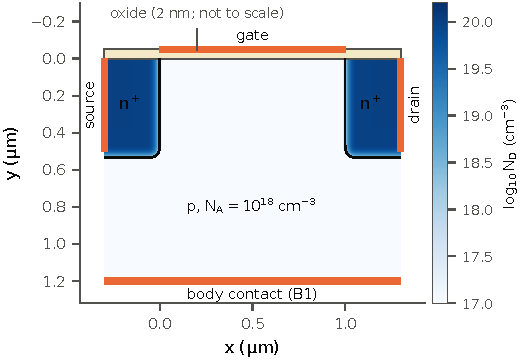
\includegraphics[width=0.62\linewidth]{figures/fig1_device.pdf}
\caption{Deck R, device dev1: donor profile of the resolved n$^+$ wells (shading; black line: metallurgical junction
$N_D = N_A$) and the contacts (orange). The oxide is drawn thicker than its 2~nm. Body contact B1 is ohmic; its
two-terminal companion B0 blocks electrons.}\label{fig:device}
\end{figure}

\Cref{tab:tiers} lists the tiers. Tier A-R and the held-out tier HO are the external-facing three-terminal sets; B-R
are their electron-blocking companions, one case per mesh. Tiers A-W and B-W use an internal, truncated deck W in which
the wells are replaced by a Dirichlet condition on a vertical segment at the well edge; standard TCAD codes cannot
reproduce it, and these tiers are kept for codes that can. Tier C
holds stress cases (gate voltages of 1~V and above, finite drain bias, well depth) with cross-path agreement only.

\begin{table}[t]
\centering\small
\caption{Benchmark tiers. $\taunum = 10^{-6}$ relative is the same-mesh tolerance.}\label{tab:tiers}
\begin{tabular}{@{}lrp{0.42\linewidth}p{0.34\linewidth}@{}}
\toprule
Tier & Cases & Content & Scored by \\
\midrule
A-R & \nAR & deck R, body B1, $\G{DD}$, $\G{SD}$ ($\G{DB}$ reported) & tolerance on any mesh; $\taunum$ on a published mesh \\
HO & \nHO & held-out deck-R states, level-1 mesh & $\taunum$ on the published mesh \\
B-R & \nBR & body-B0 companions of every A-R and HO state & same-mesh Rayleigh bracket \\
A-W & \nAW & deck W (internal) & tolerance and same-mesh bracket \\
B-W & \nBW & deck-W deep-subthreshold states & same-mesh bracket \\
C & \nC & stress: $V_G \ge 1$~V, well depth, finite bias & where established \\
\bottomrule
\end{tabular}
\end{table}

\subsection{Meshes}
Every reference mesh is a published tensor-product mesh whose rectangles are split into two triangles by a stated rule;
the node lines are given exactly (\texttt{meshes/*.json}), so a box-integration Scharfetter--Gummel code can rebuild the
identical network and declare a same-mesh submission. Three levels are published per device; the level-1 meshes have
\meshDevOneLevOne{} (dev1) and \meshDevTwoLevOne{} (dev2) silicon nodes, the level-2 meshes \meshDevOneLevTwo{} and
\meshDevTwoLevTwo{}.

% ---------------------------------------------------------------------------------------------------------------
\section{Reference values and their uncertainty}\label{sec:reference}

\subsection{Three computational paths}
\textbf{P1, network.} The equilibrium of \cref{eq:dd} is solved with DEVSIM~\cite{Sanchez2022} by Newton's method on the
published mesh. The network of \cref{eq:edge} is assembled from that equilibrium, solved by sparse LU factorization, and
evaluated in the forms of \cref{sec:discrete}, at levels 0, 1 and 2.
\textbf{P4, independent finite volume.} A separate code that imports only NumPy and SciPy, with its own tensor mesh,
box-integration assembly, damped-Newton equilibrium and network. It shares no code with P1, but it was written by the
same author for the same problem statement: it is independent in implementation, not in authorship.
\textbf{P2, drift--diffusion.} DEVSIM solves the full coupled problem at $V_D = \pm0.1$ and $\pm1$~mV with a circuit voltage
source on the drain. The current is taken in three ways: DEVSIM's post-solve contact current, the current of the circuit
voltage source, and a weighting-function current. Central differences $G(\delta) = [I(\delta) - I(-\delta)]/2\delta$ are
combined as $G_R = [100\,G(0.1~\mathrm{mV}) - G(1~\mathrm{mV})]/99$.

\subsection{Pre-registered acceptance}
The primary states, the held-out states and every threshold were fixed before the first production run; amendments
were dated and appended, and none changed a state, threshold or tolerance rule. A primary state (H1) had to satisfy,
for $\G{DD}$ and $\G{SD}$, $|P4/P1_{L2} - 1| \le 5\times10^{-3}$, $|P1_{L2}/P1_{L1} - 1| \le 5\times10^{-3}$, agreement of
the two forms and current conservation within $10^{-9}$, and the B0 bracket at every level; the tier was to be withdrawn
if fewer than 4 of 6 states passed. All \HonePass{} passed; the largest P4 difference was \maxPfour{} and the largest
level-2 to level-1 change \maxRefine{}. All \HtwoPass{} held-out states passed their criteria (forms and conservation
within $10^{-9}$, bracket). In the drift--diffusion runs, the circuit-node current's Richardson value agreed with the P1
network within \ecircWorst{} in all \nPtwoRuns{} runs.

\subsection{Tolerances}
The reference value of an A-R state is P1 on the level-2 mesh. Its tolerance, applied separately to $\G{DD}$ and
$\G{SD}$, is $2\,(u_\mathrm{disc} + u_\mathrm{round} + u_\mathrm{solver})$, where
$u_\mathrm{disc} = \max(|P1_{L2}/P1_{L1} - 1|, |P4/P1_{L2} - 1|)$, $u_\mathrm{round}$ is the spread of the two forms and
$u_\mathrm{solver}$ the network residual. It ranges from \tolMin{} to \tolMax{} (\cref{tab:states}). On a published mesh
the same-mesh reference is exact to round-off and a submission is held to $\taunum = 10^{-6}$. Because the P4 spread is
part of the tolerance, P4 passes by construction: that is a consistency check, not independent validation.
\Cref{fig:refs} shows the range of the references.

\textbf{Grid convergence.} A three-grid analysis of the P1 values at levels 0, 1 and 2~\cite{Roache1994,Celik2008}, with
the refinement ratio taken from the node counts (about 1.41 per level), supports these tolerances (\cref{tab:gci}). It
was pre-registered with three predictions, all of which hold. Convergence is monotone in all \gciMonotone{} of
\gciPairs{} cases (six states, $\G{DD}$ and $\G{SD}$), with observed orders \gciPmin{}--\gciPmax{}, as expected of a
second-order scheme. Farrell and Peschka found second-order convergence of the Scharfetter--Gummel finite-volume current
for smooth doping, and only first-order convergence of their finite-volume potential for near-discontinuous
doping~\cite{FarrellPeschka2019}; our wells have smooth erfc profiles. The asymptotic-range ratio is \gciAsymMin{}--\gciAsymMax{} (1 in the asymptotic range). The
level-2 references lie \gciRelMin{} to \gciRelMax{} from the Richardson-extrapolated values; the registered tolerances
contain these differences by a factor of \gciTolRatioMin{} to \gciTolRatioMax{}, and contain the grid convergence index
of the finest mesh (\gciFineMin{} to \gciFineMax{}) in \gciFineWithin{} of \gciPairs{} cases. In \gciPfourCloser{} of \gciStates{} states the independent
finite-volume value lies closer to the extrapolated value (within \gciPfourMax{}) than the finest network value does.

\begin{table}[t]
\centering\small
\caption{Three-terminal reference values (body B1). A-R values are P1 at level 2, with the relative tolerance for any
mesh; HO values are the level-1 same-mesh references.}\label{tab:states}
\begin{tabular}{@{}llrrrrrr@{}}
\toprule
State & Device & $V_G$ (V) & $\hat\psi$ & $G_{DD}$ (S/cm) & $G_{SD}$ (S/cm) & $\Delta L$ (nm) & Tolerance \\
\midrule
AR-1 & dev1 & 0.488174 & 12.0 & \num{3.5276e-12} & \num{3.5041e-12} & 34.21 & \num{2.8e-3} \\
AR-2 & dev1 & 0.621433 & 16.0 & \num{1.6162e-10} & \num{1.6160e-10} & 38.52 & \num{3.7e-3} \\
AR-3 & dev1 & 0.7835 & 21.0 & \num{2.1098e-8} & \num{2.1098e-8} & 40.84 & \num{4.7e-3} \\
AR-4 & dev2 & 0.488174 & 12.0 & \num{2.5502e-9} & \num{2.5451e-9} & 364.23 & \num{2.6e-4} \\
AR-5 & dev2 & 0.621433 & 16.0 & \num{1.2034e-7} & \num{1.2033e-7} & 381.53 & \num{2.5e-4} \\
AR-6 & dev2 & 0.7835 & 21.0 & \num{1.5974e-5} & \num{1.5974e-5} & 395.18 & \num{2.4e-4} \\
\midrule
HO-1 & dev1 & 0.588534 & 15.0 & \num{6.1776e-11} & \num{6.1753e-11} & 37.92 & $\tau_\mathrm{num}$ only \\
HO-2 & dev1 & 0.686557 & 18.0 & \num{1.1211e-9} & \num{1.1211e-9} & 39.54 & $\tau_\mathrm{num}$ only \\
HO-3 & dev2 & 0.588534 & 15.0 & \num{4.5692e-8} & \num{4.5687e-8} & 377.87 & $\tau_\mathrm{num}$ only \\
HO-4 & dev2 & 0.686557 & 18.0 & \num{8.4012e-7} & \num{8.4011e-7} & 388.06 & $\tau_\mathrm{num}$ only \\
HO-5 & dev1, $L = 2\,\mu$m & 0.488174 & 12.0 & \num{1.7171e-12} & \num{1.6840e-12} & 29.38 & $\tau_\mathrm{num}$ only \\
\bottomrule
\end{tabular}

\end{table}

\begin{table}[t]
\centering\small
\caption{Grid convergence of the A-R references ($\G{DD}$; $\G{SD}$ agrees to two digits): observed order $p$, distance of
the level-2 value from the extrapolated value, grid convergence index of the finest mesh (safety factor 1.25), registered
tolerance, and distance of the independent finite-volume value (P4) from the extrapolated value.}\label{tab:gci}
\begin{tabular}{@{}lrrrrr@{}}
\toprule
State & $p$ & $|G_{L2}/G_\mathrm{ext} - 1|$ & $\mathrm{GCI}_\mathrm{fine}$ & Tolerance & $|G_{P4}/G_\mathrm{ext} - 1|$ \\
\midrule
AR-1 & 2.21 & \num{1.3e-3} & \num{1.6e-3} & \num{2.8e-3} & \num{1.6e-4} \\
AR-2 & 2.22 & \num{1.6e-3} & \num{2.0e-3} & \num{3.7e-3} & \num{2.3e-4} \\
AR-3 & 2.21 & \num{2.0e-3} & \num{2.5e-3} & \num{4.7e-3} & \num{2.9e-4} \\
AR-4 & 2.02 & \num{1.2e-4} & \num{1.4e-4} & \num{2.6e-4} & \num{1.5e-5} \\
AR-5 & 2.00 & \num{1.2e-4} & \num{1.5e-4} & \num{2.5e-4} & \num{6.0e-6} \\
AR-6 & 1.98 & \num{1.2e-4} & \num{1.5e-4} & \num{2.4e-4} & \num{1.9e-5} \\
\bottomrule
\end{tabular}

\end{table}

\begin{figure}[t]
\centering
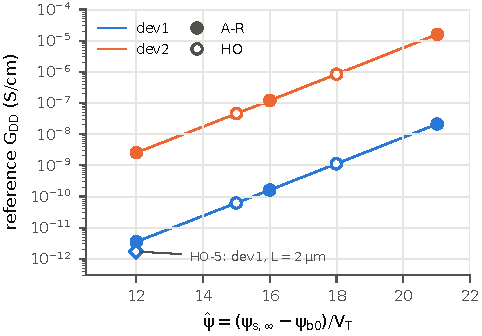
\includegraphics[width=0.55\linewidth]{figures/fig2_references.pdf}
\caption{Reference $\G{DD}$ against the long-channel band bending $\hat\psi$ for dev1 and dev2 (filled: A-R; open: HO).
The drain current at 1~mV is $\G{DD}\times 1$~mV, from \IoneMin{} to \IoneMax{}~A/cm.}\label{fig:refs}
\end{figure}

% ---------------------------------------------------------------------------------------------------------------
\section{Scorer and submission format}\label{sec:scorer}
A submission is a JSON file that maps case identifiers to values (\texttt{G\_DD\_S\_per\_cm}, \texttt{G\_SD\_S\_per\_cm}, or
$G_0$) and may declare \texttt{same\_mesh} with a published mesh identifier. The scorer applies, in order: a sign
check (a conductance $\le 0$ fails); for a same-mesh three-terminal submission, $|G/G_\mathrm{ref} - 1| \le \taunum$
against the reference on that mesh; for any other A-R submission, the tolerance of \cref{tab:states} and the matching
$\Delta L$ tolerance; for two-terminal same-mesh submissions, the Rayleigh bracket with a relative slack of $10^{-12}$.
A case with no applicable check is reported as not scorable. \Cref{tab:examples} lists the worked examples shipped with
the benchmark: each re-submits an evaluation path from the production records through the unchanged scorer.

\begin{table}[t]
\centering\small
\caption{Worked examples: evaluation paths submitted to the scorer (cases passed and failed).}\label{tab:examples}
\begin{tabular}{@{}lrr@{}}
\toprule
Submitted evaluation path & Pass & Fail \\
\midrule
Reference forms (A-R, HO), same mesh & 11 & 0 \\
DEVSIM circuit-node current $-x[\mathrm{V1.I}]$, Richardson, same mesh & 11 & 0 \\
Independent finite volume (A-R), other mesh & 6 & 0 \\
DEVSIM \texttt{get\_contact\_current}, double, Richardson, same mesh & 0 & 11 \\
DEVSIM \texttt{get\_contact\_current}, extended precision (A-R) & 6 & 0 \\
Coupled small-signal solve $G_E$ (full Jacobian), level-1 mesh & 0 & 11 \\
DEVSIM AC analysis, double (A-R) & 0 & 6 \\
DEVSIM AC analysis, extended precision (A-R) & 0 & 6 \\
\midrule
Two-terminal source-side reference, same mesh & 86 & 0 \\
Two-terminal drain-side flux sum, same mesh & 48 & 38 \\
Two-terminal coupled small-signal $G_E$, same mesh & 0 & 14 \\
Two-terminal independent finite volume (A-W), other mesh & 3 & 0 \\
\bottomrule
\end{tabular}

\end{table}

% ---------------------------------------------------------------------------------------------------------------
\section{Failure-mode atlas}\label{sec:atlas}
\Cref{fig:atlas} summarizes the error of each evaluation path against the same-mesh reference on the level-1 mesh, as a
function of the size of the current. The scope of every statement in this section is these devices, these meshes and
DEVSIM~2.11.2.

\begin{figure}[t]
\centering
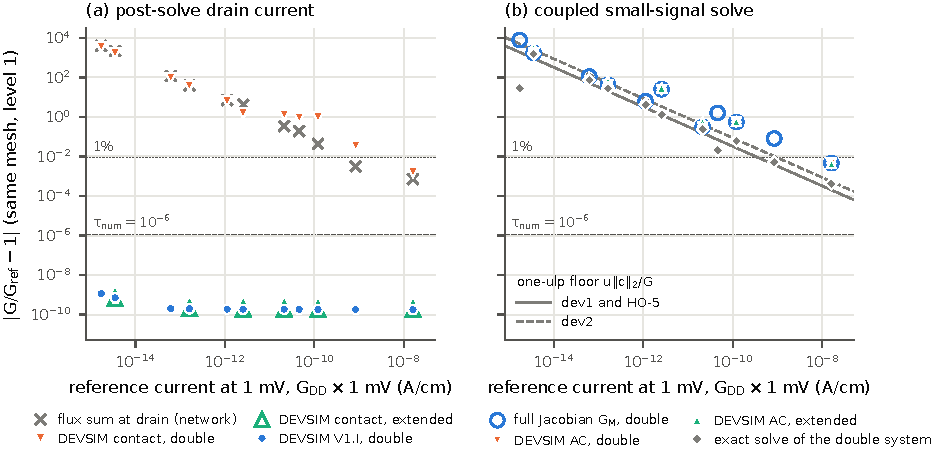
\includegraphics[width=\linewidth]{figures/fig3_atlas.pdf}
\caption{Relative error of $\G{DD}$ from each evaluation path, against the size of the current, for the 11 A-R and HO
states on their level-1 meshes (body B1). (a) Post-solve currents, Richardson values $G_R$ of the drain current (DEVSIM
paths), and the drain-side flux sum of the network itself. (b) The coupled small-signal solve of the full Jacobian,
DEVSIM's AC analysis (A-R states), and the exact solution of the same double-precision system (diamonds, all 11
states). Gray lines: the one-ulp data floor $u\|c\|_2/G$ of each device (exploratory analysis, \cref{sec:ss}); HO-5
shares the floor of dev1.
Dashed: $\taunum$; dotted: 1\%.}\label{fig:atlas}
\end{figure}

\subsection{Flux sum at the excited contact}
Summing the edge currents at the drain contact of the network itself, rather than using an energy or source-side form,
misses the same-mesh reference by more than $\taunum$ on every A-R and HO mesh, and by up to \fluxMax{} relative, with the
wrong sign, at $\hat\psi = 12$ (\cref{fig:atlas}a, crosses). The source-side sum of the same solution is exact to
round-off. The error is a round-off effect, not a discretization error: it does not decrease under mesh refinement, while
the source-side and energy forms of the same solution agree to $10^{-9}$ or better. We did not analyse its mechanism
further.

\subsection{DEVSIM's post-solve contact current}\label{sec:post}
A related failure appears in DEVSIM's default contact current (\texttt{get\_contact\_current}) of a full
drift--diffusion solution. Its absolute error, measured against the circuit-node current of the same runs, was
\floorMin{} to \floorMax{}~A/cm on these meshes. On the dev1 level-1 mesh at $V_D = +0.1$~mV the raw drain current was
\identValue{}~A/cm, identical to all digits, in \identN{} runs (\identStates) whose $\G{DD}$ spans \identGlo{} to
\identGhi{}~S/cm: below about $10^{-11}$~A/cm the value carries no channel information. Pre-registered predictions of
the error at $\pm1$~mV (above $10^{-2}$ where $\G{DD}\times1$~mV $\le 10^{-10}$~A/cm, below it where $\ge 10^{-8}$~A/cm)
were confirmed for all \pddConfirmed{} predicted states, and, scored as a submission, this current failed all
\hthreeAll{} scorable cases (\cref{fig:atlas}a, triangles). Two remedies pass: the circuit-node current, whose Richardson
value matched the reference within \ecircWorst{} in all runs, and DEVSIM's extended precision
(\texttt{extended\_solver}, \texttt{extended\_model}, \texttt{extended\_equation}), with which the contact current equalled
the circuit-node current to double-precision resolution and its Richardson value matched the reference within
\extMaxRich{} in \extPass{} of \extN{} A-R states, at \extCostMin{}--\extCostMax{} times the wall time.

\subsection{The coupled small-signal solve and DEVSIM's AC analysis}\label{sec:ss}
The linear-response problem can also be posed on the full coupled Jacobian of \cref{eq:dd} at equilibrium, as
small-signal analysis does: solve $J\,\delta x = \delta b$, where $\delta b$ is the change of the residual for a drain-bias
step, and read the conductance from the circuit unknown of the drain voltage source. We solved this system with two sparse direct
solvers, SuperLU after row and column equilibration ($G_E$) and UMFPACK through DEVSIM's interface ($G_M$). The solves
reach a normwise backward error of at most \etaMax{}, yet $G_E$ and $G_M$ were wrong by up to \pssMaxGE{} and \pssMaxGM{}
relative. The componentwise condition number of the output with respect to the entries of $J$,
$\kappa_J = \sum_{ij}|\lambda_i J_{ij}\,\delta x_j|/|G|$ with $\lambda = J^{-\mathsf{T}}e$ the adjoint solution for the
circuit unknown (the device form of the adjoint method of network sensitivity analysis~\cite{GhioneFilicori1993}) and
$G$ the reference, was \xsKappaMin{} to \xsKappaMax{}. The pre-registered prediction that
$G_E$ misses by more than 1\% in the \pssPredicted{} dev1 states was confirmed in \pssConfirmed{}. A small backward error does
not imply a small forward error when the output is this ill-conditioned~\cite{Higham2002}; the practical point is that a
residual check alone accepts this output.

DEVSIM's built-in AC analysis (\texttt{solve(type='ac')}, here at $10^{-6}$~Hz) is this same solve: its drain current
reproduced $G_M$ bit for bit in \acBitwise{} of \acN{} A-R states. It failed in all \acN{} states in double precision
(error up to \acMaxDouble{}) and in all \acN{} in extended precision (up to \acMaxExt{}). Extended precision cannot help
here because, in DEVSIM~2.11.2, the AC system is factored and solved once in double precision even when the DC solution
is extended (source code inspection, recorded with the release).

\textbf{The data, not the solver.} A pre-registered follow-up asked whether the error comes from the rounding of the
factorization or from the double-precision system itself. The system of each of the \ssStates{} states was rebuilt (bit
for bit, in all \ssRepro{}) and solved exactly: iterative refinement with residuals accumulated in double-double
arithmetic and the solution held in double-double~\cite{Higham2002,Demmel2006} converged in at most \ssIterMax{} steps to a componentwise backward error of at most
\ssOmegaMax{}, and two inner solvers gave the same solution to \ssMbMax{}. The exact solution of the double-precision
system was still wrong in every state, by \ssExactMin{} (AR-6, the largest current) to \ssExactMax{} relative
(\cref{fig:atlas}b, diamonds). The exact solve left \ssShareOneMin--\ssShareOneMax\% of the
double-precision error on dev1, \ssShareTwoMin--\ssShareTwoMax\% on dev2 and \ssShareThree\% on HO-5. Multiplying every
entry of $J$ by $1 + 2^{-52}u$, with $u$ uniform on $[-1, 1]$ and three seeds, moved $G$ by \ssSdblMin--\ssSdblMax\% of
the double-precision error. Both registered predictions therefore failed: that the exact solve removes 99\% of the error (true in
\ssPMoneOk{} of \ssGate{} states with an error above 1\%) and that one-ulp rounding of the entries moves $G$ by less than
1\% of it (\ssPMtwoOk{} of \ssGate{}). As fixed in advance, this means that the double-precision Jacobian does not
determine the conductance at these currents: no double-precision solver can repair the output. Refinement returns
the solution of the stored system and takes its entries as exact~\cite{Demmel2006}; it cannot recover what their
rounding has lost.

\textbf{Where the sensitivity lies (exploratory).} This analysis was specified after the first records were seen and
before it was run, without predictions. To first order, relative changes $\rho_{ij}$ of the entries change the output by
$\sum_{ij} c_{ij}\rho_{ij}$, with $c_{ij} = \lambda_i J_{ij}\,\delta x_j$ computed from the exact $\lambda$ and $\delta x$.
This linear response reproduced the measured one-ulp shifts to \xsLinearMax{}, with second-order terms below
\xsSecondMax{} of them. In every state at least \xsDrainMin\% of $\sum|c_{ij}|$ lies in the electron-continuity rows of
the drain-side n-type region, and at least \xsColsPotMin\% in the potential columns. (DEVSIM's unknowns are the
potential and the electron density, the variables Selberherr recommends for computation~\cite[Sec.~5.2]{Selberherr1984}.)
In the neutral drain the potential
follows the drain voltage ($\delta\psi_j = 1$), every current injected there leaves through the drain ($\lambda_i = 1$ to
within \xfLamDev{} on AR-1 and AR-4), and the Jacobian entries of these rows reach \xsEntryMax{}~S/cm on the thin cells
at the surface. The Scharfetter--Gummel flux depends on the potential only through differences, so the potential entries
of each such row sum to zero; the stored entries do so to within \xfRowSumMax{} of their absolute sum (AR-1, AR-4). The large terms of each row
therefore cancel, and the rounding of each entry leaves a current that the drain collects. Its size, $u\|c\|_2$ with
$u = 2^{-53}$, is fixed by the drain region and does not depend on the gate bias (within \xsFloorSpread{} relative in all states of a
device): \xsFloorOne{}~S/cm on dev1,
\xsFloorTwo{} on dev2 and \xsFloorThree{} on the longer dev1 of HO-5 (\cref{fig:atlas}b, gray lines). The errors of the
exact solves were \xsActMin{} to \xsActMax{} times this floor. Computed from the unrefined double-precision solutions,
the floor agreed with the exact one to \xsUnrefMax{}, so one adjoint solve with the same factorization estimates it
without a reference. A conductance that is not well above this floor cannot be obtained from the double-precision
Jacobian. Because the floor is proportional to the rounding of the entries, an assembly and solve in higher precision
would lower it in proportion (first-order theory, not tested here). The reference does not have this sensitivity: it
evaluates $G$ from the edge conductances in the energy form, which is stationary with respect to errors in the
potentials and, by Rayleigh's monotonicity law, changes by at most the relative rounding of the
conductances~\cite{DoyleSnell1984}. An assembly that applies each flux derivative to a potential difference may also
avoid the floor, and the nonlinear residual evaluates each flux from the potential difference, which may be why
bias-step differences of the circuit current were accurate (\cref{sec:post}); we did not test either.

This failure of the coupled small-signal output, with a backward error near machine precision, was not found in the
literature we reviewed; adjoint and Green's-function formulations of small-signal and noise analysis are
established~\cite{GhioneFilicori1993}, and we have not read all small-signal literature.


\subsection{Recommendations for users}
For currents or current differences below a few times $10^{-9}$~A/cm on meshes like these, where the absolute error
floor reaches \floorMax{}~A/cm: do not trust a post-solve contact flux in double precision; use the circuit-node current, a weighting-function or energy form, or extended precision. Do not accept a
small-signal output because its residual is small, nor because it was refined: compare it with a finite difference of
converged DC solutions or with a cancellation-free form, and estimate its data floor $u\|c\|_2$ from one adjoint solve. Check every low-current result against an evaluation that does not subtract at the
excited contact.

% ---------------------------------------------------------------------------------------------------------------
\section{AI-agent study}\label{sec:agents}

\subsection{Question and design}
Does an LLM agent, asked to compute a low-current conductance with an open simulator, report a wrong value as correct
when it cannot use the scorer? The study was pre-registered~\cite{Nosek2018} and its protocol frozen after two smoke runs
on a non-benchmark state and before the first study run. Each run was a fresh, headless Claude Code session (version
2.1.318) on the model \texttt{claude-opus-5-5} with effort ``high'', a 150-turn limit and a 2700~s wall limit. The tools
were limited to shell, file read/write/edit and search; there were no web tools, MCP servers, skills, subagents, project
documents or memory. A workspace guard refused access outside the run's own workspace, and Claude Code's automatic
permission mode reviewed every tool call.

The \agentRuns{} runs of arm A cover the 11 A-R and HO states, three repeats each, in a seeded order. Each workspace held a
neutral device description, the level-1 mesh, the converged equilibrium as arrays, a DEVSIM deck that rebuilds the device
with a circuit source on the drain, the DEVSIM manual and its examples. The prompt asked for $\G{DD} = \partial I_D/\partial V_D$
at $V_D = 0$ ``within 1\% of the exact value for this device and mesh'' and for a final JSON block with the value, a status
(success, uncertain or failed), the method and the verification. The reference values were never in the workspace. A
run is a \emph{silent error} (SE) if it claims success with a value outside 1\% of the same-mesh reference; the other
outcomes are correct and claimed (CS), flagged error (FE), flagged correct (FC) and no report (NR). The primary metric
is the SE rate with a Clopper--Pearson interval~\cite{ClopperPearson1934}. Arm B, with a checker returning pass or fail
within 1\% (at most three calls), was to follow only if arm A produced at least one SE: the registered stop rule
reports a negative result otherwise. Every transcript was audited for access outside the workspace and for leaked
reference material.

\subsection{Results}
All \agentRuns{} arm-A runs were valid (none contaminated, none with a harness failure). There were \agentSE{} silent
errors, \agentCS{} correct and claimed, \agentFE{} flagged errors, \agentFC{} flagged correct and \agentNR{} without a
report (\cref{tab:agent,fig:agents}). The SE rate is 0/\agentRuns{}, with a 95\% upper bound of \agentSEhi{}; the CS rate
is \agentCSrate{} (95\% interval \agentCSlo--\agentCShi). The \agentNreported{} reported values had a median relative
error of \agentMedianRel{} and a largest of \agentMaxRel{}. The run without a report reached the wall limit while an
extended-precision check on the largest task mesh (dev2, level 1) was still running; the values already in its log
were within 1\%. The median wall time was \agentMedianWall~s (\agentWallLow~s for the \agentLow{} low-current runs,
\agentWallModerate~s for the \agentModerate{} moderate ones). By the registered stop rule, arm B was not run.

\begin{table}[t]
\centering\small
\caption{Agent study, arm A: outcomes of the three runs per task and the largest relative error of the reported values.
$G_\mathrm{ref}$ is the same-mesh reference on the level-1 mesh; ``low'' means $G_\mathrm{ref}\times1$~mV $\le 10^{-10}$~A/cm.}\label{tab:agent}
\begin{tabular}{@{}lllrlr@{}}
\toprule
Task & State & Class & $G_\mathrm{ref}$ (S/cm) & Outcomes & max $|\epsilon|$ \\
\midrule
T01 & AR-1 & low & \num{3.533e-12} & CS CS CS & \num{1.1e-4} \\
T02 & AR-2 & low & \num{1.619e-10} & CS CS CS & \num{2.6e-5} \\
T03 & AR-3 & low & \num{2.115e-8} & CS CS CS & \num{1.1e-5} \\
T04 & AR-4 & low & \num{2.550e-9} & CS CS CS & \num{2.8e-6} \\
T05 & AR-5 & moderate & \num{1.204e-7} & CS CS CS & \num{1.5e-5} \\
T06 & AR-6 & moderate & \num{1.598e-5} & CS CS NR & \num{2.1e-5} \\
T07 & HO-1 & low & \num{6.178e-11} & CS CS CS & \num{9.9e-5} \\
T08 & HO-2 & low & \num{1.121e-9} & CS CS CS & \num{1.7e-5} \\
T09 & HO-3 & low & \num{4.569e-8} & CS CS CS & \num{5.4e-5} \\
T10 & HO-4 & moderate & \num{8.401e-7} & CS CS CS & \num{2.1e-5} \\
T11 & HO-5 & low & \num{1.717e-12} & CS CS CS & \num{3.4e-5} \\
\bottomrule
\end{tabular}

\end{table}

\begin{figure}[t]
\centering
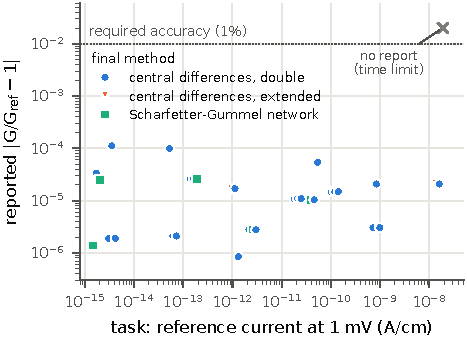
\includegraphics[width=0.55\linewidth]{figures/fig4_agents.pdf}
\caption{Agent study, arm A: relative error of the \agentNreported{} reported values against the size of the current, by
the final method each agent reported (three runs per task, offset horizontally). The cross marks the run that reached the
time limit without a report.}\label{fig:agents}
\end{figure}

What the agents did is described from the transcripts; this description was not pre-registered and decides nothing.
Every run called DEVSIM's contact current (\agentCalledContact/\agentRuns) and \agentCalledAC{} ran its AC analysis,
the two failing paths of \cref{sec:atlas}; \agentExtended{} used extended precision.
By their own method statements, the final methods were central differences of a converged DC current in double
precision (\methodA{} runs) or in extended precision (\methodB), or an exact linearization on the Scharfetter--Gummel
network (\methodC). Every reporting run checked its value independently: \verifCurrent{} of the \agentNreported{}
statements of verification describe a second current measure (edge-current sums across channel cuts, the network against
the finite difference, or the contact currents for the moderate-current task), and one an estimate from the sheet
electron density. Several runs named the failing paths and why they
were rejected, for example (run W6-004): ``DEVSIM's built-in AC solve (6.6e-8) and get\_contact\_current are dominated by rounding
error at the 1e20~cm$^{-3}$ contacts and were rejected.''

\subsection{Sensitivity and deviations}
Before the twelfth run, an audit rule was corrected by a dated amendment: a tool call that was refused and never executed
no longer counts as an access, and the agent's own Claude Code scratch directory is not forbidden. Under the audit as
frozen, \sensOrigContaminated{} runs count as contaminated; in each the flagged call reads the agent's own background-task
output and was refused by Claude Code before it ran, and each reported a correct value. The registered worst case counts
contaminated runs as SE; with the frozen audit it gives \sensWorstSE/\agentRuns{} (95\% interval
\sensWorstLo--\sensWorstHi), under which the stop rule would not apply. The decision follows the primary analysis, as
registered, and the primary analysis gives zero SE under either audit. Other deviations, recorded with the release, did
not affect any outcome: two runs were started above the usage cap agreed in advance, the cloud host restarted between
queue sessions, and a transient outage of the permission classifier refused \refusedClassifier{} tool calls in one run.
In total \refusedCalls{} tool calls in \refusedRuns{} runs were refused; none of them sought project files, other runs or
the reference values.

\subsection{Interpretation}
For this agent, kit and prompt, the silent error that the benchmark is built to catch did not occur in \agentRuns{} runs.
The failing paths were reached in every run and set aside each time, after the agent checked its value independently;
the methods it chose are those the benchmark identifies as accurate. The result does not show
that agents in general avoid this error. The conditions favour detection: the prompt states the 1\% requirement and asks
for a status; the deck makes the circuit current one call away; the documentation is local; one model and one configuration
were tested; and the model under test is the one that designed the study (see the disclosure below). The null result does
not transfer to agents with default system prompts, other models, tasks without a stated accuracy, or users who build the
deck themselves.

% ---------------------------------------------------------------------------------------------------------------
\section{Discussion}\label{sec:discussion}
\textbf{Use.} The A-R tier can score any drift--diffusion code that implements the scope of \cref{tab:scope}: compute the
$V_D \to 0$ conductances on any mesh and compare with the tolerance, or rebuild a published mesh and compare with
$\taunum$. The held-out and two-terminal tiers and the worked examples test the evaluation of the current in isolation.
The atlas gives the signatures to look for: an error that does not scale with the mesh, a value independent of the gate
voltage, a residual that is clean while the output is not.

\textbf{Limits.} All agreement reported here is between computational paths; nothing is validated against experiment, and
the physics envelope is narrow (Boltzmann statistics, constant mobility, no holes in the observable, no recombination,
zero or small $V_D$). The independent finite-volume path is independent in implementation but shares the model, the
problem statement and the author. The reference equilibrium of P1 comes from DEVSIM, and the only external code scored is DEVSIM; an
evaluation of NiTCAD~\cite{NiTCAD}, whose documentation describes a weighted terminal current with an error estimate, is on
hold because the code targets Windows and its build requires a dependency version we could not obtain. $\G{DB}$ and the held-out and
B-R cases have no tolerance usable on other meshes. The analysis of where the small-signal sensitivity lies is
exploratory and covers DEVSIM's Jacobian on these meshes only. The agent study tested one model in one configuration.

\textbf{Relation to prior work.} The benchmark complements the diode benchmark of Farrell and Peschka~\cite{FarrellPeschka2019}
in device (MOSFET), regime (subthreshold, linear response) and output (terminal conductance), and uses their test-function
view of the current. The flux-integration failure it quantifies is classical~\cite{PalmVandeWiele1985}; the benchmark
contributes a modern, scored quantification in an open tool and a remedy check, not a new mechanism. The cancellation
traced in \cref{sec:ss} is its linear-response counterpart: in both, a small current is formed from large terms in the
heavily doped region, once in the flux at the contact and once in the Jacobian rows of the neutral drain. We did not find
the second described in the literature we reviewed, which includes the standard monograph on device
simulation~\cite{Selberherr1984}, the adjoint approach to small-signal sensitivity and noise~\cite{GhioneFilicori1993}
and extra-precise iterative refinement~\cite{Demmel2006}.

% ---------------------------------------------------------------------------------------------------------------
\section{Conclusions}
We release an open, pre-registered verification benchmark for the low-current, linear-response terminal conductances of
two-dimensional MOSFETs with resolved wells, with tolerances usable by any code, published meshes, a scorer and worked
examples. Scored against it, DEVSIM's default post-solve contact current fails in every scorable case because of a
round-off floor of order $10^{-11}$~A/cm, and its AC analysis fails because the coupled small-signal solve is ill-conditioned
while its residual is clean; extended precision repairs the first and not the second. The second is a property of the
double-precision Jacobian, not of the solver, since an exact solve of the same system fails too. An exploratory analysis
traces it to the neutral drain, where the potential derivatives of the fluxes cancel and their rounding leaves a floor of
a few $10^{-9}$~S/cm, the size of the errors of the exact solves. An LLM agent working without the
scorer set aside DEVSIM's contact current in all \agentRuns{} runs and its AC analysis in all \agentCalledAC{} runs that
used it, and reported no wrong value as correct. The benchmark's value for
agents and users who do not check their low currents independently remains to be tested under harder conditions.

\section*{Data and code availability}
The benchmark (case files, meshes, schema, scorer, worked examples), the production records and evaluation scripts of
every work package, the agent-study transcripts and audits, and the sources of this manuscript are released with this
paper: code under the MIT License and data, text and figures under CC BY 4.0
([repository URL and Zenodo DOI to be added on release]). Every result quoted in this manuscript (numbers, tables and figures) is
generated from the released files by \texttt{paper/scripts/make\_assets.py}; their SHA-256 are listed in \texttt{paper/generated/inputs.sha256}.
Design parameters (states, thresholds, limits) are those of the pre-registrations released with the data.

\section*{Use of AI}
This study was planned, implemented, run and analysed, and this manuscript was drafted, by Claude (Anthropic, model
\texttt{claude-opus-5-5}) working as an AI research assistant under the direction of the author, who set the research
direction and made the decisions recorded in the pre-registrations. [To be confirmed by the author: the author has reviewed the manuscript and
takes responsibility for its content.] The agent under test in \cref{sec:agents} is the same model, run separately with a fixed
configuration; that the model under test also designed the study is a potential source of bias.

\bibliographystyle{unsrtnat}
\bibliography{references}

\end{document}
